\chapter{Lterature Survey} 
\thispagestyle{plain} 
Storm is a free and open source distributed real time computation system. Storm makes it easy to reliably process unbounded streams of data, doing for realtime processing what Hadoop did for batch processing. Storm is simple, can be used with any programming language.
Storm has many use cases: realtime analytics, online machine learning, continuous computation, distributed RPC, ETL, and more. Storm is fast: a benchmark clocked it at over a million tuples processed per second per node. It is scalable, fault-tolerant, guarantees your data will be processed, and is easy to set up and operate.
\begin{center}
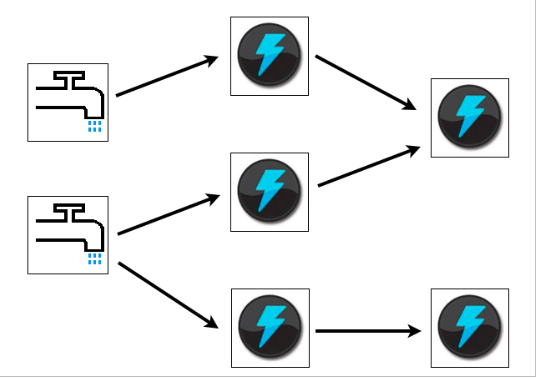
\includegraphics[scale=.5]{../img/img4} \\[2mm]
\end{center}
Storm integrates with the queueing and database technologies we already use. A Storm topology consumes streams of data and processes those streams in arbitrarily complex ways, repartitioning the streams between each stage of the computation however needed.The work is delegated to different types of components that are each responsible for a simple specific processing task. The input stream of a Storm cluster is handled by a component called a spout. The spout passes the data to a component called a bolt, which transforms it in some way. A bolt either persists the data in some sort of storage, or passes it to some other bolt. One can imagine a Storm cluster as a chain of bolt components that each make some kind of transformation on the data exposed by the spout.\\[2mm]
{\bfseries Processing streams} \\[2mm]
As demonstrated in the preceding example, unlike other stream processing systems,
with Storm there’s no need for intermediate queues.\\[2mm]
{\bfseries Continuous computation} \\[2mm]
Send data to clients continuously so they can update and show results in real time,
such as site metrics.\\[2mm]
{\bfseries Distributed remote procedure call} \\[2mm]
Easily parallelize CPU-intensive operations
\subsection*{Storm Architecture} 
\begin{center}
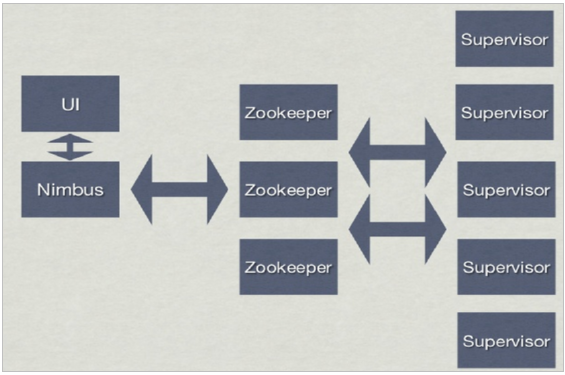
\includegraphics[scale=.5]{../img/img5} \\[2mm]
\end{center}
{\bfseries Nimbus:} This node runs a daemon process called Nimbus. Nimbus is responsible for distributing code across the cluster, assigning tasks to machines, and monitoring the success and failure of units of work.\\[2mm]
{\bfseries Worker nodes:} These nodes run a daemon process called the Supervisor. A Supervisor is responsible for listening for work assignments for its machine. It then subsequently starts and stops worker processes. Each worker process executes a subset of a topology, so that the execution of a topology is spread across a multitude of worker processes running on a multitude of machines.\\[2mm]
Sitting between the Nimbus and the various Supervisors is the Apache open source project {\bfseries ZooKeeper}.\\[2mm] 
ZooKeeper's goal is to enable highly reliable distributed coordination, mainly by acting as a centralized service for distributed cluster functionality.
Storm topologies are deployed to the Nimbus and then the Nimbus deploys spouts and bolts to Supervisors. When it comes time to execute spouts and bolts, the Nimbus communicates with the Supervisors by passing messages to Zookeepers. Zookeepers maintain all state for the topology, which allows the Nimbus and Supervisors to be fail-fast and stateless: if the Nimbus or Supervisor processes go down then the state of processing is not lost; work is reassigned to another Supervisor and processing continues. Then, when the Nimbus or a Supervisor is restarted, they simply rejoin the cluster and their capacity is added to the cluster.
\begin{center}
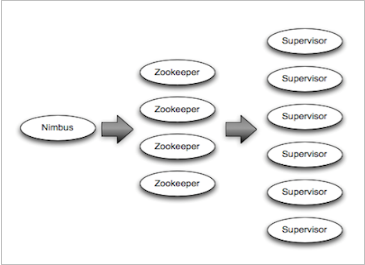
\includegraphics[scale=1]{../img/img6}\\[2mm]
\end{center}

